\documentclass{beamer}

\mode<presentation> {

%\usetheme{default}
%\usetheme{AnnArbor}
%\usetheme{Antibes}
%\usetheme{Bergen}
%\usetheme{Berkeley}
%\usetheme{Berlin}
%\usetheme{Boadilla}
%\usetheme{CambridgeUS}
%\usetheme{Copenhagen}
%\usetheme{Darmstadt}
%\usetheme{Dresden}
%\usetheme{Frankfurt}
%\usetheme{Goettingen}
%\usetheme{Hannover}
%\usetheme{Ilmenau}
%\usetheme{JuanLesPins}
%\usetheme{Luebeck}
\usetheme{Madrid}
%\usetheme{Malmoe}
%\usetheme{Marburg}
%\usetheme{Montpellier}
%\usetheme{PaloAlto}
%\usetheme{Pittsburgh}
%\usetheme{Rochester}
%\usetheme{Singapore}
%\usetheme{Szeged}
%\usetheme{Warsaw}


%\usecolortheme{albatross}
%\usecolortheme{beaver}
%\usecolortheme{beetle}
%\usecolortheme{crane}
%\usecolortheme{dolphin}
%\usecolortheme{dove}
%\usecolortheme{fly}
%\usecolortheme{lily}
%\usecolortheme{orchid}
%\usecolortheme{rose}
%\usecolortheme{seagull}
%\usecolortheme{seahorse}
%\usecolortheme{whale}
%\usecolortheme{wolverine}

%\setbeamertemplate{footline} % To remove the footer line in all slides uncomment this line
%\setbeamertemplate{footline}[page number] % To replace the footer line in all slides with a simple slide count uncomment this line

%\setbeamertemplate{navigation symbols}{} % To remove the navigation symbols from the bottom of all slides uncomment this line
}

\usepackage{graphicx} % Allows including images
\usepackage{booktabs} % Allows the use of \toprule, \midrule and \bottomrule in tables
\usepackage{amsfonts}
\usepackage{mathrsfs}
\usepackage{amsmath,amssymb,graphicx, bm}
\usepackage{dirtytalk} % quote thing

%----------------------------------------------------------------------------------------
%	TITLE PAGE
%----------------------------------------------------------------------------------------

\title["8.4"]{8.4: Multivariate ARMA Processes}

\author{Taylor} 
\institute[UVA] 
{
University of Virginia \\
\medskip
\textit{} 
}
\date{} 

\begin{document}
%----------------------------------------------------------------------------------------

\begin{frame}
\titlepage 
\end{frame}
%----------------------------------------------------------------------------------------

\begin{frame}
\frametitle{Motivation}

In this section we introduce ARMA models for vectors $\mathbf{X}_t$.

\end{frame}

%----------------------------------------------------------------------------------------

\begin{frame}
\frametitle{Example 8.4.1}

a vector-valued AR(1).
\[
\mathbf{X}_t = \bm{\Phi} \mathbf{X}_{t-1} + \mathbf{Z}_t, \hspace{10mm} \mathbf{Z}_t \sim WN(0,\Sigma)
\]
or
\[
\left[\begin{array}{c}
X_{t,1} \\
X_{t,2}
\end{array}\right] =
\left[\begin{array}{cc}
\bm{\Phi}_{11} & \bm{\Phi}_{12} \\
\bm{\Phi}_{21} & \bm{\Phi}_{22}
\end{array}\right]
\left[\begin{array}{c}
X_{t-1,1} \\
X_{t-1,2}
\end{array}\right]  +
\left[\begin{array}{c}
Z_{t,1} \\
Z_{t,2}
\end{array}\right] 
\]
or
\begin{align*}
X_{t,1} &= \bm{\Phi}_{11} X_{t-1,1} + \bm{\Phi}_{12} X_{t-1,2} + Z_{t,1} \\
X_{t,2} &= \bm{\Phi}_{21} X_{t-1,1} + \bm{\Phi}_{22} X_{t-1,2} + Z_{t,2} 
\end{align*}



\end{frame}



%----------------------------------------------------------------------------------------

\begin{frame}
\frametitle{Example 8.4.1}


\begin{align*}
\mathbf{X}_t &= \bm{\Phi} \mathbf{X}_{t-1} + \mathbf{Z}_t \\
&= \bm{\Phi}^2 \mathbf{X}_{t-2} + \bm{\Phi} \mathbf{Z}_{t-1} + \mathbf{Z}_t \\
&= \bm{\Phi}^3 \mathbf{X}_{t-3} + \bm{\Phi}^2 \mathbf{Z}_{t-2} + \bm{\Phi} \mathbf{Z}_{t-1} + \mathbf{Z}_t\\
&\vdots \\
&= \sum_{j=1}^{\infty} \bm{\Phi}^j Z_{t-j}
\end{align*}
as long as the eigenvalues of $\bm{\Phi}$ are less than $1$.


\end{frame}


%----------------------------------------------------------------------------------------

\begin{frame}
\frametitle{Example 8.4.1}


Why does $\bm{\Phi}^k \mathbf{X}_{t-k} \to \mathbf{0}$ as long as the eigenvalues of $\bm{\Phi}$ are less than $1$?
\newline

Assume for simplicity that the eigenvectors $q_1, q_2, \ldots, q_n$ are linearly independent (the proof is more complicated if they are not). We can write 
\[
\bm{\Phi} q_i = \lambda_i q_i
\]
as
\[
\bm{\Phi}Q   = Q \Lambda 
\]
or
\[
\bm{\Phi} = Q \Lambda Q^{-1}
\]
where $Q = [\begin{array}{cccc}q_1 & q_2 & \cdots & q_n \end{array}]$ and $\Lambda = \text{diag}(\lambda_1, \ldots, \lambda_n)$. 
\newline

Finally, notice that $\bm{\Phi}^k = Q \Lambda^k Q^{-1} \to Q \mathbf{0} Q^{-1} = \mathbf{0}$.


\end{frame}

%----------------------------------------------------------------------------------------

\begin{frame}
\frametitle{Example 8.4.1}

$q_i \neq 0$ is an eigenvector with eigenvalue $\lambda_i < 1$ iff
\[
\bm{\Phi} q_i = \lambda_i q_i
\]
iff
\[
(I\lambda_i - \bm{\Phi}) q_i = 0
\]
iff
\[
\det(I\lambda_i - \bm{\Phi}) = 0
\]
iff
\[
\det(I - \bm{\Phi}z) = 0  \hspace{10mm} z = 1/\lambda_i> 0
\]
\pause
The last equation is the determinant of a matrix-valued polynomial.

\end{frame}

%----------------------------------------------------------------------------------------

\begin{frame}
\frametitle{Definition}

\begin{block}{Vector ARMA}
$\{\mathbf{X}_t\}$ is an {\bf ARMA(p,q) process} if $\{\mathbf{X}_t\}$ is stationary and if for every $t$,
\[
\mathbf{X}_t - \bm{\Phi}_1 \mathbf{X}_{t-1} - \cdots - \bm{\Phi}_p \mathbf{X}_{t-p} = \mathbf{Z}_{t} + \bm{\Theta}_1\mathbf{Z}_{t-1} + \cdots + \bm{\Theta}_q\mathbf{Z}_{t-q},
\]
where $\{\bm{Z}_t\} \sim \text{WN}(0, \bm{\Sigma})$. $\{\mathbf{X}_t\}$ is an ARMA(p,q) process with mean $\bm{\mu}$ if $\{\mathbf{X}_t-\bm{\mu}\}$ is an ARMA(p,q) process.
\end{block}

We can write $\bm{\Phi}(B) \mathbf{X}_t = \bm{\Theta} \mathbf{Z}_t$ where $\bm{\Phi}(z) = I - \bm{\Phi}_1 z - \cdots \bm{\Phi}_pz^p$ and $\bm{\Theta}(z) = I + \bm{\Theta}_1 z  + \cdots + \bm{\Theta}_q z^q$.
\end{frame}


%----------------------------------------------------------------------------------------

\begin{frame}
\frametitle{Definition}

\begin{block}{Causal Vector ARMA model}
An ARMA(p,q) process $\{\mathbf{X}_t\}$ is {\bf causal} if there exist matrices $\{\bm{\Psi_j}\}$ with absolutely summable components such that 
\[
\mathbf{X}_t = \sum_{j=0}^{\infty} \bm{\Psi}_j \mathbf{Z}_{t-j} \hspace{10mm} \text{for all } t.
\]
Equivalently:
\[
\det(\bm{\Phi}(z)) \neq 0 \text{ for all } z \in \mathbb{C} \text{ such that } |z| \le 1.
\]
\end{block}


\end{frame}

%----------------------------------------------------------------------------------------

\begin{frame}
\frametitle{Definition}

\begin{block}{Invertible Vector ARMA model}
An ARMA(p,q) process $\{\mathbf{X}_t\}$ is {\bf invertible} if there exist matrices $\{\bm{\Pi_j}\}$ with absolutely summable components such that 
\[
\mathbf{Z}_t = \sum_{j=0}^{\infty} \bm{\Pi}_j \mathbf{X}_{t-j} \hspace{10mm} \text{for all } t.
\]
Equivalently:
\[
\det(\bm{\Theta}(z)) \neq 0 \text{ for all } z \in \mathbb{C} \text{ such that } |z| \le 1.
\]
\end{block}
\pause

These definitions are analagous to the univariate case. Roots outside are good!


\end{frame}

%----------------------------------------------------------------------------------------

\begin{frame}
\frametitle{Remark}

Can a vector AR(1) be equivalent to a vector MA(1)? This isn't possible for univariate ARMA models. Hint: consider the vector-AR(1) model with $\bm{\Phi} = \left[ \begin{array}{cc} 0 & .5 \\ 0 & 0 \end{array}\right]$.
\newline
\pause

There is no identifiability problem if you restrict your attention to AR models (VAR models). From now on, we only deal with these.




\end{frame}

%----------------------------------------------------------------------------------------

\begin{frame}
\frametitle{Theoretical ACF of causal VAR models}

For a causal VAR model
\[
\mathbf{X}_t = \sum_{j=0}^{\infty} \bm{\Psi}_j \mathbf{Z}_{t-j},
\]
the ACF is
\[
\Gamma(h) = \sum_{j=0}^{\infty}\bm{\Psi}_{j+h} \bm{\Sigma} \bm{\Psi}_{j}.
\]

\end{frame}

%----------------------------------------------------------------------------------------

\begin{frame}
\frametitle{Applied Example}

See code for a VAR modelling example.
\begin{center}
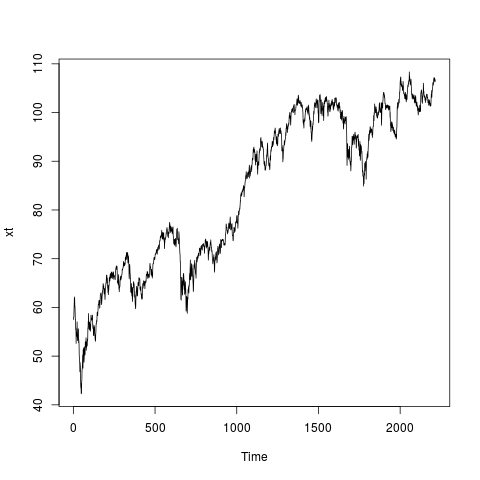
\includegraphics[width=70mm]{/home/taylor/UVa/all_teaching/4170_slides/8/8.4/Rplot.png}
\end{center}

\end{frame}



\end{document} 